\documentclass[tikz,border=7pt]{standalone}
\usepackage{amsmath,amssymb}
\usetikzlibrary{arrows.meta,calc}

\definecolor{regionexact}{HTML}{DCEBE8}
\definecolor{regioncapacity}{HTML}{F2E4C8}
\definecolor{regioncurve}{HTML}{DDE6F3}
\definecolor{regionhead}{HTML}{E4EEDC}
\definecolor{regionlocal}{HTML}{EFE1EA}
\definecolor{regionneutral}{HTML}{E8E8E6}
\definecolor{ink}{HTML}{263238}
\definecolor{mutedink}{HTML}{5C686D}
\definecolor{critical}{HTML}{B33A3A}

\begin{document}
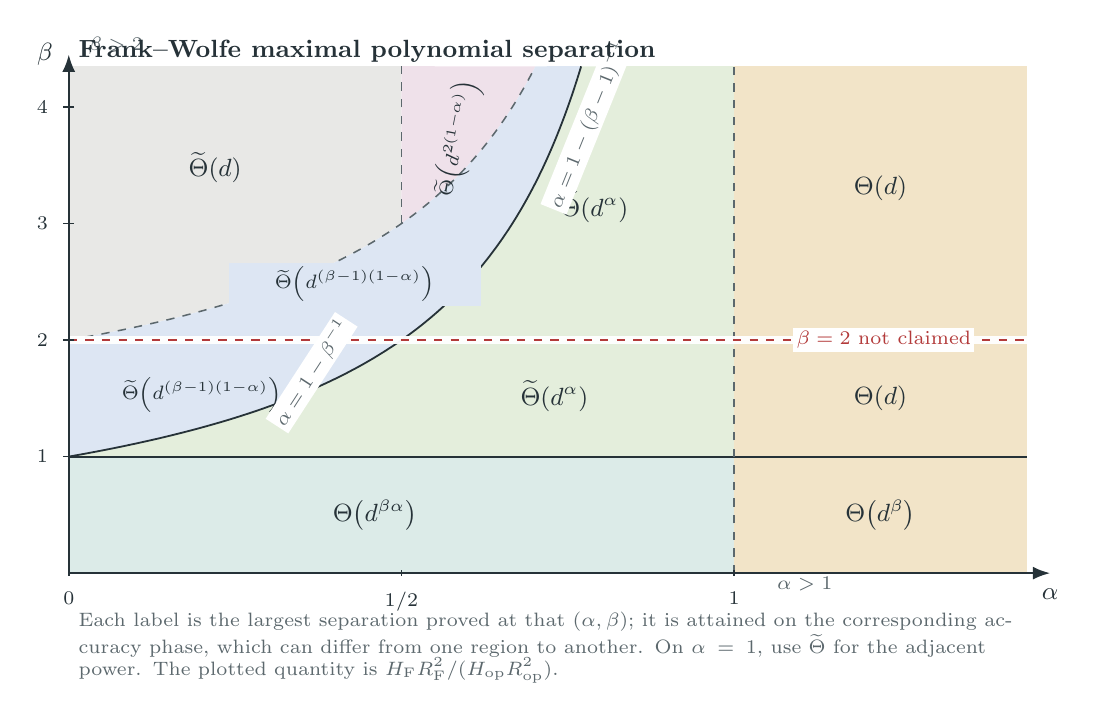
\begin{tikzpicture}[
  x=8.45cm,
  y=1.48cm,
  >=Latex,
  axis/.style={draw=ink, line width=0.75pt, -{Latex[length=2.2mm]}},
  boundary/.style={draw=ink, line width=0.65pt},
  softboundary/.style={draw=mutedink, line width=0.55pt, dashed},
  formula/.style={text=ink, align=center, font=\small},
  smallformula/.style={text=ink, align=center, font=\scriptsize},
  note/.style={text=mutedink, align=left, font=\scriptsize}
]
  \def\amax{1.44}
  \def\bmax{4.35}

  % Polynomial-phase regions below beta=2.
  \fill[regionexact] (0,0) rectangle (1,1);
  \fill[regioncapacity] (1,0) rectangle (\amax,1);
  \fill[regioncurve]
    (0,1)
    -- plot[domain=1:2,samples=80] ({1-1/\x},{\x})
    -- (0,2) -- cycle;
  \fill[regionhead]
    (0,1) -- (1,1) -- (1,2) -- (0.5,2)
    -- plot[domain=2:1,samples=80] ({1-1/\x},{\x})
    -- cycle;
  \fill[regioncapacity] (1,1) rectangle (\amax,2);

  % Strongest fixed-polynomial phase established above beta=2.
  \fill[regionneutral]
    (0,2)
    -- plot[domain=2:3,samples=80] ({1-1/(\x-1)},{\x})
    -- (0.5,\bmax) -- (0,\bmax) -- cycle;
  \fill[regionlocal]
    (0.5,3)
    -- plot[domain=3:\bmax,samples=80] ({1-1/(\x-1)},{\x})
    -- (0.5,\bmax) -- cycle;
  \fill[regioncurve]
    (0,2)
    -- plot[domain=2:\bmax,samples=120] ({1-1/(\x-1)},{\x})
    -- plot[domain=\bmax:2,samples=120] ({1-1/\x},{\x})
    -- cycle;
  \fill[regionhead]
    (0.5,2)
    -- plot[domain=2:\bmax,samples=120] ({1-1/\x},{\x})
    -- (1,\bmax) -- (1,2) -- cycle;
  \fill[regioncapacity] (1,2) rectangle (\amax,\bmax);

  % Region boundaries.
  \draw[boundary] (0,1) -- (\amax,1);
  \draw[boundary]
    plot[domain=1:\bmax,samples=150] ({1-1/\x},{\x});
  \draw[softboundary]
    plot[domain=2:\bmax,samples=130] ({1-1/(\x-1)},{\x});
  \draw[softboundary] (0.5,3) -- (0.5,\bmax);
  \draw[softboundary] (1,0) -- (1,\bmax);

  % The critical capacity is intentionally left open.
  \fill[white,opacity=0.96] (0,1.965) rectangle (\amax,2.035);
  \draw[critical,line width=0.75pt,dashed] (0,2) -- (\amax,2);
  \node[fill=white,inner sep=1.2pt,text=critical,font=\scriptsize]
    at (1.225,2) {$\beta=2$ not claimed};

  % Axes and ticks.
  \draw[axis] (0,0) -- (\amax+0.035,0)
    node[below=2pt,text=ink,font=\small] {$\alpha$};
  \draw[axis] (0,0) -- (0,\bmax+0.10)
    node[left=2pt,text=ink,font=\small] {$\beta$};
  \foreach \a/\lab in {0/0,0.5/{1/2},1/1}
    \draw[ink,line width=0.55pt] (\a,0.025) -- (\a,-0.025)
      node[below=2pt,text=ink,font=\scriptsize] {$\lab$};
  \foreach \b in {1,2,3,4}
    \draw[ink,line width=0.55pt] (0.008,\b) -- (-0.008,\b)
      node[left=2pt,text=ink,font=\scriptsize] {$\b$};
  \node[text=mutedink,font=\scriptsize,anchor=west] at (1.05,-0.09) {$\alpha>1$};
  \node[text=mutedink,font=\scriptsize,anchor=south west] at (0.015,4.37) {$\beta>2$};

  % Separation labels. Every label is a pure power of d.
  \node[formula] at (0.46,0.50) {$\Theta\!\left(d^{\beta\alpha}\right)$};
  \node[formula] at (1.22,0.50) {$\Theta\!\left(d^{\beta}\right)$};

  \node[smallformula,text width=3.2cm] at (0.20,1.53)
    {$\widetilde\Theta\!\left(d^{(\beta-1)(1-\alpha)}\right)$};
  \node[formula] at (0.73,1.52)
    {$\widetilde\Theta\!\left(d^{\alpha}\right)$};
  \node[formula] at (1.22,1.50) {$\Theta(d)$};

  \node[formula] at (0.22,3.48) {$\widetilde\Theta(d)$};
  \node[smallformula,rotate=79] at (0.585,3.73)
    {$\widetilde\Theta\!\left(d^{2(1-\alpha)}\right)$};
  \node[smallformula,fill=regioncurve,inner sep=1.5pt,text width=3.1cm]
    at (0.43,2.48)
    {$\widetilde\Theta\!\left(d^{(\beta-1)(1-\alpha)}\right)$};
  \node[formula] at (0.79,3.14)
    {$\widetilde\Theta\!\left(d^{\alpha}\right)$};
  \node[formula] at (1.22,3.30) {$\Theta(d)$};

  % Boundary labels and interpretation notes.
  \node[note,fill=white,inner sep=1pt,rotate=57]
    at (0.365,1.72) {$\alpha=1-\beta^{-1}$};
  \node[note,fill=white,inner sep=1pt,rotate=68]
    at (0.78,3.85) {$\alpha=1-(\beta-1)^{-1}$};

  \node[anchor=north west,text=ink,font=\bfseries\small]
    at (0,\bmax+0.31)
    {Frank--Wolfe maximal polynomial separation};
  \node[anchor=north west,note,text width=12.0cm]
    at (0,-0.25)
    {Each label is the largest separation proved at that $(\alpha,\beta)$;
     it is attained on the corresponding accuracy phase, which can differ
     from one region to another.  On $\alpha=1$, use $\widetilde\Theta$ for the adjacent power.  The plotted quantity is
     $H_{\mathrm F}R_{\mathrm F}^{2}/(H_{\mathrm{op}}R_{\mathrm{op}}^{2})$.};

\end{tikzpicture}
\end{document}
